\begin{figure}[t]
\centering
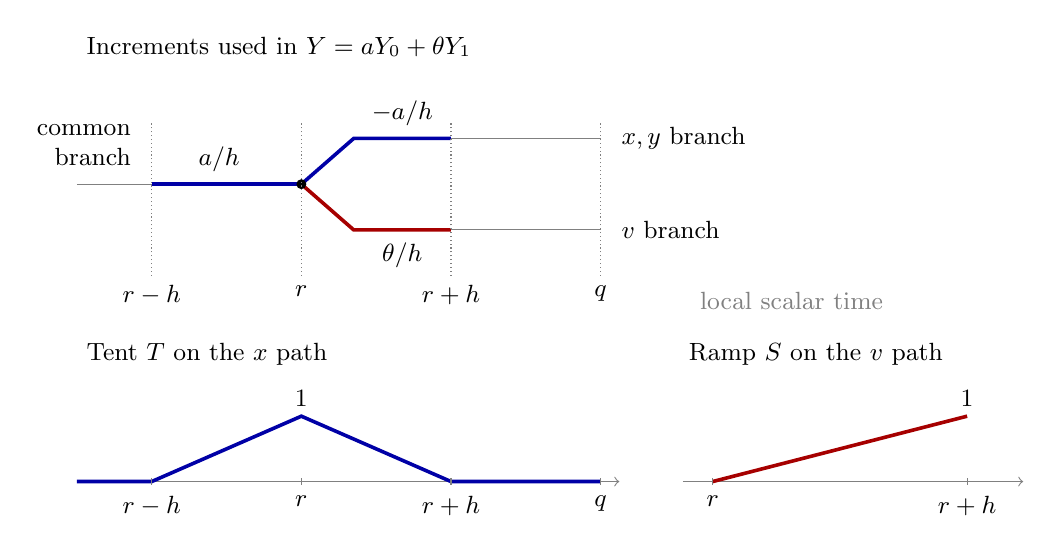
\begin{tikzpicture}[x=0.95cm,y=0.83cm,
  every node/.style={font=\small},
  active/.style={line width=1.3pt,blue!65!black},
  other/.style={line width=1.3pt,red!65!black}]
  \node[anchor=west] at (0,5.00) {Increments used in $Y=aY_0+\theta Y_1$};
  \draw[gray] (0,2.9)--(3,2.9);
  \draw[active] (1,2.9)--(3,2.9);
  \draw[active] (3,2.9)--(3.7,3.6)--(5,3.6);
  \draw[gray] (5,3.6)--(7,3.6);
  \draw[other] (3,2.9)--(3.7,2.2)--(5,2.2);
  \draw[gray] (5,2.2)--(7,2.2);
  \fill (3,2.9) circle[radius=1.8pt];
  \node[above] at (1.9,2.94) {$a/h$};
  \node[above] at (4.35,3.65) {$-a/h$};
  \node[below] at (4.35,2.15) {$\theta/h$};
  \node[anchor=west] at (7.15,3.6) {$x,y$ branch};
  \node[anchor=west] at (7.15,2.2) {$v$ branch};
  \node[anchor=east,align=right] at (0.85,3.50) {common\\branch};
  \foreach \x/\t in {1/{r-h},3/r,5/{r+h},7/q} {
    \draw[gray,densely dotted] (\x,1.5)--(\x,3.85);
    \node[below] at (\x,1.5) {$\t$};
  }
  \node[anchor=west,text=gray] at (8.2,1.12) {local scalar time};

  \node[anchor=west] at (0,0.30) {Tent $T$ on the $x$ path};
  \draw[->,gray] (0,-1.65)--(7.25,-1.65);
  \draw[active] (0,-1.65)--(1,-1.65)--(3,-0.65)
                       --(5,-1.65)--(7,-1.65);
  \node[above] at (3,-0.65) {$1$};
  \foreach \x/\t in {1/{r-h},3/r,5/{r+h},7/q} {
    \draw[gray] (\x,-1.60)--(\x,-1.70);
    \node[below] at (\x,-1.72) {$\t$};
  }

  \node[anchor=west] at (8.05,0.30) {Ramp $S$ on the $v$ path};
  \draw[->,gray] (8.1,-1.65)--(12.65,-1.65);
  \draw[other] (8.5,-1.65)--(11.9,-0.65);
  \node[above] at (11.9,-0.65) {$1$};
  \foreach \x/\t in {8.5/r,11.9/{r+h}} {
    \draw[gray] (\x,-1.60)--(\x,-1.70);
    \node[below] at (\x,-1.72) {$\t$};
  }
\end{tikzpicture}
\caption{The three increments in the perturbation. The upper labels are
coefficients of the raw field increments in $Y$; $a=1-\theta$.
Horizontal position records local scalar time, not the mass-sorted order
of the hierarchy. Below, the raw covariance of $Y_0$ with $X_s^x$,
divided by $\beta^2$, is the tent $T(s)$, which vanishes before the
endpoint $q$. Conditional on the common field $X_r$, the raw covariance
of $Y_1$ with $X_s^v$ on $[r,r+h]$, divided by $\beta^2$, is the ramp
$S(s)$. The tent isolates the small change in Parisi mass near $r$;
the other branch supplies the mixed susceptibility term. Lengths are
schematic.}
\label{fig:narrow-increments}
\end{figure}
